\documentclass[12pt]{report}
\usepackage[utf8]{inputenc}
\usepackage{tabularx} % extra features for tabular environment
\usepackage{amsmath,amssymb,amsthm}  % improve math presentation
\usepackage{algorithm2e}
\usepackage{caption}
\usepackage{subcaption}
\newcommand{\E}{\mathrm{E}}
\newcommand{\Var}{\mathrm{Var}}
\newcommand{\Cov}{\mathrm{Cov}}
\newcommand{\Cor}{\mathrm{Cor}}
\DeclareMathOperator*{\argmin}{argmin}
\DeclareMathOperator*{\argmax}{argmax}
\newcommand\norm[1]{\left\lVert#1\right\rVert}
\newcommand\myleqa{\mathrel{\overset{\makebox[0pt]{\mbox{\normalfont\tiny\sffamily (a)}}}{\leq}}}
\newcommand\myleqb{\mathrel{\overset{\makebox[0pt]{\mbox{\normalfont\tiny\sffamily (b)}}}{\leq}}}
\newcommand\myleqc{\mathrel{\overset{\makebox[0pt]{\mbox{\normalfont\tiny\sffamily (c)}}}{\leq}}}
\newcommand\myeqa{\mathrel{\overset{\makebox[0pt]{\mbox{\normalfont\tiny\sffamily (a)}}}{=}}}
\newcommand\myeqb{\mathrel{\overset{\makebox[0pt]{\mbox{\normalfont\tiny\sffamily (b)}}}{=}}}
\usepackage{graphicx} % takes care of graphic including machinery
\usepackage[margin=1in,letterpaper]{geometry} % decreases margins
\usepackage{cite} % takes care of citations
\usepackage[final]{hyperref} % adds hyper links inside the generated pdf file
\hypersetup{
	colorlinks=true,       % false: boxed links; true: colored links
	linkcolor=black,        % color of internal links
	citecolor=black,        % color of links to bibliography
	filecolor=magenta,     % color of file links
	urlcolor=blue         
}
\usepackage{setspace}
\doublespacing

\begin{document}

\title{
{
\includegraphics[width=0.7\columnwidth]{university.jpg}}\\
{Greedy Principal Flows}\\
{\large National University of Singapore}\\
}
\author{Sebastian Lie}
\date{05 March 2021}
\maketitle

\chapter*{Acknowledgements}
My 7 soft toys. And my desk lamp for being the light of my life.

\chapter*{Abstract}
Principal Flows are a great tool to use when we want to extend the 
notion of Principal Component analysis to multivariate datasets that 
we know lie on non-linear manifolds. 
We restrict this problem to constructing principal flows on hyperspheres. 
We use a different, easier method to obtain the principal flow 
that is even closer to its canonical PCA interpretation. 

\newpage
\tableofcontents
\newpage

\chapter{Introduction}

\section{Motivation}

With the advent of Big Data, and the rise of data science,
machine learning has been used successfully to solve a variety of problems, 
such as regression and classification problems. However, machine learning
can also be used in a more subtle, but no less important way: to discover patterns
in the data and glean more information from it. Among methods that have this aim, 
Principal Component Analysis is the most popular, taught in almost every
machine learning course. It does however, have a glaring weakness: it does 
not perform well when the data we are working with is sampled from a non-linear manifold. 
This, however is fixed with the principal flow algorithm: 
it constructs a curve that at each local point moves in the direction of
maximal variation and retains canonical PCA interpretation in euclidean space.
Yet, this method is not easy to obtain, having to solve a problem in variational calculus. 
What if we could construct this curve with a greedy approach? 

\newpage

\section{Notation}

\begin{table}[h]
\begin{tabular}{|l|l|}
\hline
\textbf{Notation} & \textbf{Explanation}                                      \\ \hline
$\mathbb{R}^D$    & $D$ dimensional euclidean space.                      \\ \hline
$\mathbf{X}$        & Data matrix of dimensions $n \times D$                       \\ \hline
$D$                & Dimension of the high-dimensional data.                \\ \hline
$d$               & Dimension of the manifold embedded in $D$ dimensional space \\ \hline
$\mathcal{M}^d$      & Denotes a connected and complete $d$-dimensional manifold
                   embedded in $\mathbb{R}^D$                                 \\ \hline
$p$               & A point on the manifold, $\mathcal{M}^d$.            \\ \hline
$\mathbf{v}$        & A vector.                                         \\ \hline
$T_p\mathcal{M}$    & The Tangent space of a point $p$ on $\mathcal{M}^d$.   \\ \hline
$\mathbf{C}$        & A Covariance matrix.                               \\ \hline
$\{x_1,...x_n\}$  & A collection of $n$ data points in $D$ dimensions.   \\ \hline
$\mathbf{1}$      & A vector of $1$s.                                   \\ \hline
$\mathbf{I}$      & The identity matrix.                               \\ \hline
$\mathbf{X}^T$    & Transpose of a some matrix $\mathbf{X}$.                 \\ \hline
$\mathbf{X}_{(d)}$    & Transpose of a some matrix $\mathbf{X}$.               \\ \hline
$\mathbf{M}$    & Dissimilarity Matrix, dimension $n \times n$                  \\ \hline
\end{tabular}
\end{table}

\newpage

\section{Definitions}

\subsection{Vector Fields}
A vector at point $\mathbf{x}$, $\mathbf{x} \in \mathbb{R}^{D}$ is a pair 
$\mathbf{a} = (\mathbf{x}, \mathbf{v}), \ \mathbf{v} \in \mathbb{R}^{D}$, 
such that $\mathbf{v}$ is the vector $\mathbf{v}$ translated 
so that its tail is at $\mathbf{x}$ instead of the origin. 
All vector operations are defined such that the first item of the pair remains the same, 
and the second item is the result of the operation. 
The length and angle between two vectors are the same 
as normal vectors rooted in the origin.\\
\textbf{Definition:} A \textit{vector field} $\mathbf{F}$ on 
$U \subset \mathbb{R}^{D}$ is a function which assigns to each point
of $U$ a vector at that point. Then
$$\mathbf{F}(\mathbf{x}) = (\mathbf{x}, F(\mathbf{x}))$$ for some function 
$F: U \longrightarrow \mathbb{R}^{D}$. Vector fields on 
$\mathbb{R}^{D}$ are often most easily described by 
specifying this associated function $F$.
A pictoral example of a vector field is below.
\begin{figure}[h]
    \begin{center}
        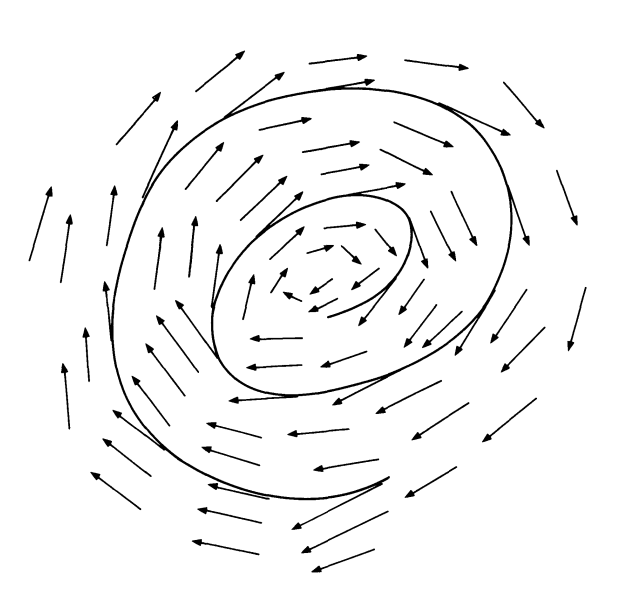
\includegraphics[scale=0.5]{fig2.5.PNG}
        \caption{An example of a vector field, $\mathbb{R}^3$}
        \label{fig:vectorfield}
    \end{center}
\end{figure}

\newpage

\subsection{Logarithm Maps}
\textbf{Logarithm Map:} For each $p \in \mathcal{M}^d$, let
$$log_p(x):\mathcal{M}^d\longrightarrow T_p\mathcal{M}$$
be the logarithm map. The log map is a function that projects a point $x$ 
on the manifold $\mathcal{M}^d$ onto $T_p\mathcal{M}$,
by producing a vector on $T_p\mathcal{M}$ which indicates the direction in which $p$
should move to obtain the projection of $x \in \mathcal{M}^d$ onto $T_p\mathcal{M}$.\\
\\
\textbf{Exponential Map:} For each $p \in \mathcal{M}^d$, let
$$exp_p(\mathbf{v}): T_p\mathcal{M} \longrightarrow \mathcal{M}^d$$
be the exponential map. Exponential maps are the inverse of the logarithm maps.
Let the vector $\mathbf{v}$ be the vector from $p$ to the point $t$ on $T_p\mathcal{M}$ we
wish to project onto $\mathcal{M}^d$. Then the exponential map moves along
the geodesic on $\mathcal{M}^d$ that mirrors the direction of $\mathbf{v}$
on $T_p\mathcal{M}$ and finds the projection of $t$ on $\mathcal{M}^d$.

\subsection{Tangent Space}
To define the tangent space we refer to the diagrams below.\\
\begin{figure}[h]
\centering
\begin{subfigure}{.5\textwidth}
    \centering
    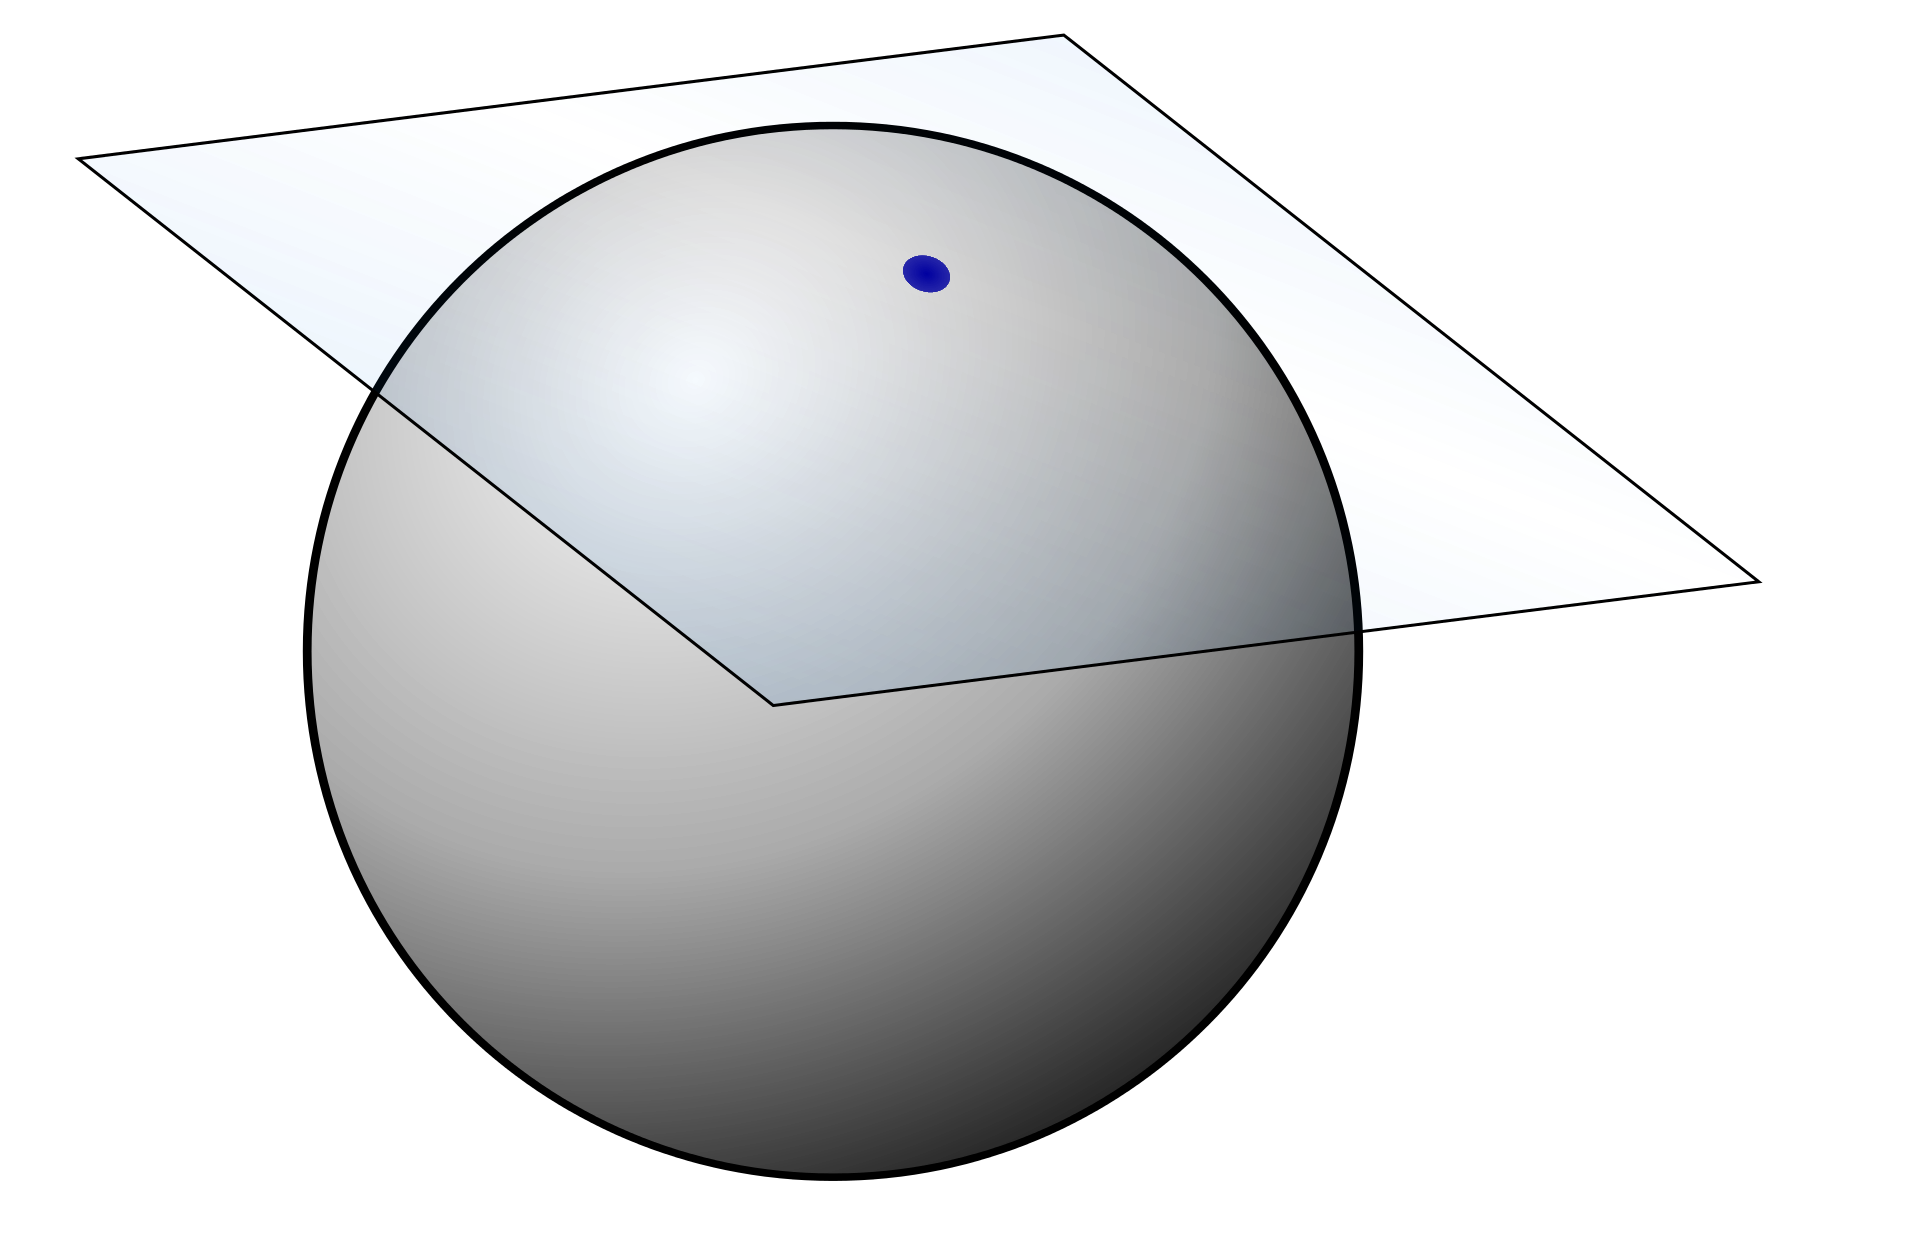
\includegraphics[scale=0.1]{tangent_space.png}
    \caption{Tangent Space of a Sphere}
    \label{tanspacesphere}
\end{subfigure}%
\begin{subfigure}{.5\textwidth}
    \centering
    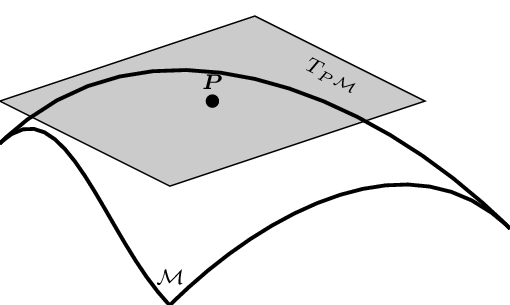
\includegraphics[scale=0.35]{tangent_space2.png}
    \caption{Close-up of the Tangent space in (a)}
    \label{tanspacemanifold}
\end{subfigure}
\caption{Illustration of a Tangent Space}
\label{fig:test}
\end{figure}
Let the sphere be the manifold, $\mathcal{M}^d$, and let $T_p\mathcal{M}$ 
be the plane tangent to $\mathcal{M}^d$. Let the blue point be $p$.
This is to say that the tangent space of some manifold $\mathcal{M}^d$
$log_p$ would then project points from $\mathcal{M}^d$ to the hyperplane,
and $exp_p$ would project points from $T_p\mathcal{M}$, the hyperplane, to $\mathcal{M}^d$.
Any vectors lying in this hyperplane are in the tangent space,
of $\mathcal{M}^d$ at $p$.


\subsection{Geodesics}

Geodesics are curves on $\mathcal{M}^d$
which play the same role as straight
lines in $\mathbb{R}^d$. They can be thought of as the "shortest path"
between 2 points on the manifold, $\mathcal{M}^d$.\\
\iffalse
or\\
\\
A geodesic on a $d$-dimensional manifold $\mathcal{M}^d \subset \mathbb{R}^D$ is a
parametrized curve $\alpha: I\longrightarrow M$ whose acceleration is everywhere
orthogonal to $\mathcal{M}^d$. Thus a geodesic is a curve in S which always goes" straight ahead" in
the surface,  Its acceleration serves only to keep it in the surface. It has no
component of acceleration tangent to the surface.\\
\fi
The Euclidean distance between 2 points $p, q$ 
is defined as $\norm{p-q}$, or the 2-norm of the vector $p - q$.
Geodesic distance extends this concept of Euclidean, straight line distance
in the Euclidean space to Manifolds. 


\subsection{Eigenvalues and Eigenvectors}
Now we define eigenvalues and eigenvectors.\\
\textbf{Definition}: Let $\mathbf{A} \in \mathbb{R}^{n \times n}$. 
Then a non-zero vector $\mathbf{v}$ is an eigenvector of $\mathbf{A}$ 
if there exists some scalar $\lambda$ such that $\mathbf{A}\mathbf{v} = \lambda \mathbf{v}$. 
Then $\lambda$ is known as the eigenvalue corresponding to vector $\mathbf{v}$.\\
Here we also note that for any 2 eigenvectors $v_i$ and $v_j$, $i \neq j$, $v_i \cdot v_j = 0$, 
or any 2 eigenvectors are orthogonal to each other, and that $v_i \cdot v_i = 1$.

\subsection{Diagonalisation}
We say that a matrix is diagonalisable if $\exists \mathbf{V}$, 
an orthonormal matrix such that the rows of $\mathbf{V}$ 
are the eigenvectors of $\mathbf{C}$, and a diagonal matrix 
$\mathbf{E}$ whose diagonal entries are the eigenvalues of $\mathbf{C}$.
In the context of this report, we only consider 
the eigendiagonalisation of some covariance matrix 
$\mathbf{C} \in \mathbb{R}^{D \times D}$,
which is symmetric and thus, always diagonalisable. Formally,
the eigendiagonalisation of $\mathbf{C}$ is given by:
$$\mathbf{C} = \mathbf{V}\mathbf{E}\mathbf{V}^T$$

\chapter{Literature Review}

\section{Linear Dimension Reduction}

\subsection{Principal Component Analysis}

\textbf{Principal Component analysis} tries to obtain a 
lower-dimensional representation of the data 
that retains as much variation as possible present in the data set. 
PCA relies on constructing principal components (PCs): 
new variables that are linear combinations of the original variables 
that have first been centered.
These PCs are uncorrelated (orthogonal) and ordered in descending order 
by the amount of variability of the original data retained.
\iffalse
Note that centering each variable is the same as finding the "mean" 
observation $\bar{x} = \frac{1}{n}\sum^n_{i=1}x_i$, 
and subtracting that from every observation: $x_i - \bar{x}$, 
since $\bar{x}_i$ is the mean of the i-th variable.
This is done by calculating the covariance matrix 
of the centered data, $\mathbf{C}$, then 
computing the eigendiagonalisation of $\mathbf{C}$ 
and compute the dot product of the original 
data matrix by the $d$ eigenvectors associated with the 
$d$ largest eigenvalues.
\fi
It reduces some high-dimensional data of dimension $D$ 
to $d$ by computing the first $d$ PCs
in the process below:\\
\begin{algorithm}[H]
    \SetAlgoLined
    \KwResult{Write here the result }
     initialization\;
     \While{While condition}{
      instructions\;
      \eIf{condition}{
       instructions1\;
       instructions2\;
       }{
       instructions3\;
      }
     }
     \caption{How to write algorithms}
    \end{algorithm}
\textbf{Algorithm}
\begin{enumerate}
    \item First we center the data matrix, $\mathbf{X}$.
    \item Next we compute the covariance matrix of 
    the centered data matrix: $\mathbf{C}$.
    \item Now we compute the eigendiagonalisation of $\mathbf{C}$,
    and obtain $\mathbf{V}_d$, the $d$ eigenvectors associated
    the $d$ largest eigenvalues.
    \item Then constructing the $d$ principal components
    is done by computing $\mathbf{X}\mathbf{V}_d$.
\end{enumerate}

\subsection{Classical MDS, Euclidean Distance}
\textbf{Multidimensional Scaling}'s 
main aim is to take some $D$ dimensional data, $\mathbf{X} \in \mathbb{R}^{n \times D}$ 
and find some $d$ dimensional points that minimises the discrepancy 
in the pairwise distances of the points in the original $D$ dimensional
representation and the new $d$ dimensional representation.\\
Let a squared dissimilarity matrix calculated using euclidean distance
between n points be given by
$\mathbf{M} \in \mathbb{R}^{n \times n}$, (define M in notation)
let the matrix of coordinates be denoted by 
$\mathbf{X} \in \mathbb{R}^{n \times D}$, 
and let $\mathbf{B} = \mathbf{X}\mathbf{X}^T$ be the gram matrix.
Since dissimilarities do not change under translations, 
we assume that $\mathbf{X}$ has column means equal to 0. 
MDS seeks to find a lower dimensional representation (define $X_{(d)}$)
$\mathbf{X}_{(d)} \in \mathbb{R}^{n \times d}$.\\
\textbf{Algorithm}:
\begin{enumerate}
    \item Compute or obtain the dissimilarity matrix, $\mathbf{S}$.
    \item Let $\mathbf{J}$ be the centering matrix: 
    $\mathbf{J} = \mathbf{I} - n^{-1}\mathbf{1}\mathbf{1}^T$. 
    Compute $\mathbf{B} = -\frac{1}{2}\mathbf{J}\mathbf{S}\mathbf{J}$.
    \item Then, compute the eigensdecomposition of $\mathbf{B}$: 
    $\mathbf{B} = \mathbf{V}\mathbf{\Lambda}\mathbf{V}^T$. 
    \item Then $\mathbf{X} = \mathbf{V}\mathbf{\Lambda}^{1/2}$ 
    and for a d-dimensional representation of 
    $\mathbf{X}$: $\mathbf{X}_{(d)}$, $\mathbf{X}_{(d)} = \mathbf{V}_d\mathbf{\Lambda}^{1/2}_d$, 
    where $\mathbf{\Lambda}^{1/2}_d$ is the first $d \times d$ submatrix of $\Lambda$,
     and $\mathbf{V}_d$ is the first $d$ columns of $\mathbf{V}$, 
     i.e the first $d$ eigenvectors and their corresponding eigenvalues.
\end{enumerate}
Note that using Euclidean distances, the result of MDS is the same as PCA.

\section{Non-Linear Dimension Reduction}

Non-linear dimensionality reduction methods are particularly useful 
when the multivariate data we obtain is sampled 
from a smooth non-linear manifold $\mathcal{M}^d$, 
e.g a manifold in an S-shape or a hypersphere. 
This class of methods obtain better estimates than linear methods like PCA and MDS,
especially for the data mentioned above. 
They are especially successful as certain data sets contain 
essential nonlinear structures that are invisible to PCA and MDS.

\newpage

\subsection{Isomap}

\textbf{Isomap}, introduced by Tenenbaum et al. \cite{isomap} is an extension 
of MDS to manifolds in which embeddings 
are optimized to preserve geodesic distances between pairs of data points.
It combines the major algorithmic features of PCA and MDS
 — computational efficiency, global optimality, 
 and asymptotic convergence guarantees — 
 with the flexibility to learn a broad class of nonlinear manifolds.
 Isomap achieves this by estimating the geodesic distance between data points, 
 given only input-space distances, e.g euclidean distance between points.\\
\\
This relies on the fact that for neighboring points, 
input-space distance provides a good approximation to geodesic distance. 
For faraway points, Isomap approximates geodesic distance 
by adding up a sequence of “short hops” between neighboring points, 
computed efficiently by finding shortest paths in a graph with edges 
connecting neighboring data points.  
This approximation relies on the proof that for a 
sufficiently high density of data points, 
we can always choose a neighborhood size (e or K) large enough 
that the graph will (with high probability) have a path not much longer 
than the true geodesic, but small enough to prevent edges 
that “short circuit” the true geometry of the manifold \cite{isomap}.\\
\textbf{Isomap Algorithm}:
\begin{enumerate}
    \item Construct neighbourhood graph $G$: 
    First, we need to compute the distances between points: 
    for any node i and j, connect the 2 nodes if 
    $d(i,j) < \epsilon$ or if j is one of the k-nearest neighbours of i.
    \item Compute all-pairs shortest paths on $G$. 
    There are many algorithms to do this, but we use the Floyd-Warshall algorithm.
    \item Construct a d-dimensional embedding using MDS.
\end{enumerate}

\newpage

\subsection{Locally Linear Embeddding}

\textbf{Locally Linear Embedding (LLE)} introduced by 
Saul and Roweis \cite{lle} aims to construct 
a mapping from the $D$ dimensional 
original points to the $d$ dimensional reconstructed points
that preserves the local configurations of each point's nearest neighbors. 
Locally, LLE assumes the embedding is linear, 
and for each data point $p \in \mathbb{R}^D$, 
LLE uses a linear combination of its $K$ nearest neighbours 
to reconstruct a lower-dimensional $p_d \in \mathbb{R}^d$. 
LLE does this by first learning some 
reconstruction weights from the $D$-dimensional data: $\mathbf{W}$ 
where $\mathbf{W}_{ij}$ represents the contribution 
of the j-th data point in reconstructing the i-th one. 
These weights obey an important symmetry: for any particular data point, 
they are invariant to rotations, rescalings, and translations 
of that data point and its neighbors.
They thus reflect intrinsic geometric properties 
of the data that are invariant to such transformations,
and therefore, we expect their characterization of local geometry in the 
original data space to be equally valid for local patches on the manifold.
This is what motivates our use of $\mathbf{W}_{ij}$ in reconstructing
the embedded manifold coordinates in $d$ dimensions. 
At the end of LLE, each $D$-dimensional observation $\mathbf{X}_i$ 
is mapped to a low dimensional vector $\mathbf{Y}_i$ 
representing global internal coordinates on the manifold.\\
\textbf{LLE Algorithm:}
\begin{enumerate}
    \item Compute the K nearest Neighbors of each original data point 
    $\mathbf{X}_i$ using euclidean distance, where K is a hyperparameter.
    \item Compute the weights $\mathbf{W}_{ij}$ that best 
    reconstruct each data point from it's neighbours 
    minimizing the \textbf{Reconstruction Error} below by constrained linear fits.
$$\varepsilon (\mathbf{W}) = \sum_i|\mathbf{X}_i - \sum_j \mathbf{W}_{ij} \mathbf{X}_j|^2$$
    \item Compute the vectors $\mathbf{Y}_i$ best 
    reconstructed by the weights $\mathbf{W}_{ij}$ 
    by choosing the $d$ dimensional coordinates of each output  
    that minimise the embedding cost function: 
    $$\Phi(\mathbf{Y}) = \sum_i |\mathbf{Y}_i - \sum_j \mathbf{W}_{ij}\mathbf{Y}_j|^2$$
    Note that $\mathbf{W}_{ij}$ here is fixed, obtained from the previous step.
\end{enumerate}

\subsection{Principal Geodesic Analysis}

Principal Geodesic Analysis(PGA) introduced here \cite{pga}, 
is a generalization of principal component analysis to manifolds. 
The main aim of PGA is to describe some data on $\mathcal{M}^d$ 
by obtaining some principal geodesics that are analogous
to principal directions in PCA: the directions along which data is
projected to obtain a principal component.
First we qualify what an intrinsic mean is.
Let $T_p\mathcal{M}$ be the tangent space of $\mathcal{M}$ 
at the intrinsic mean $p$ of the $x_i$. 
The intrinsic mean of some data $\mathbf{X}$ lying on some manifold is obtained 
by first setting the initial mean to a random data point, 
then iteratively obtaining a better estimation of the intrinsic mean 
by computing the average of the vectors obtained using the log map at 
the current mean on all data points, then taking the next estimate of the 
intrinsic mean as the projection of that average using the exponential map 
at the current estimate.\\
Instead of finding the principal geodesic however, Fletcher et al. prove that
we can approximate the $d$ geodesics along which maximal variation lies 
by projecting data from $\mathcal{M}^d$ to $T_p\mathcal{M}$ and then finding the 
$d$ eigenvectors associated with the $d$ largest eigenvalues of the 
covariance matrix of the projected data.
\iffalse
by finding a sequence of lower-dimensional subspaces, 
which on manifolds are nested geodesic submanifolds 
that maximize the projected variance of the data. 
These submanifolds are called the principal geodesic submanifolds, 
which are analogous to linear subspaces in PCA.\\
Let $U \subset T_p\mathcal{M}$ be a neighbourhood of 0 in which our data, 
$\mathbf{X}$ lies, such that projection is well defined 
for all geodesic submanifolds of $exp_p(U)$.These principal geodesic submanifolds 
are obtained by first constructing an orthonormal basis of tangent vectors 
$v_1,...,v_d \in T_p\mathcal{M}$ that span the tangent space. 
These vectors are then used to form the principal geodesic subspaces 
$H_k$ where $H_k = exp_p(V_k)$, and $V_k$ is intersection of the 
subspace spanned by vectors $1..k$ and $U$.
subspace $V_k = span(\{v_1,...,v_k\})\bigcap U$.
\fi
\\
\textbf{Algorithm}:
\begin{enumerate}
    \item Obtain the intrinsic mean, $p \in \mathcal{M}^d$ of $\{x_1,..x_n\}$.
    \item Calculate the vectors $u_i = log_p(x_i)$.
    \item Calculate the covariance matrix $\mathbf{S} = \frac{1}{n} \sum^n_{i=1} u_iu_i^T$.
    \item Diagonalise the covariance matrix to obtain $\{v_k, \lambda_k\}$ 
    the eigenvectors and eigenvalues respectively, 
    which represent the principal directions in the tangent space $T_p\mathcal{M}$ and the variances.
\end{enumerate}


\chapter{Greedy Principal Flows}

\section{Goal Of Research}

The main objective for greedy principal flows is to quantify or describe 
multivariate data on the manifold: we cannot simply fit a line, 
as this is not Euclidean space.
Instead, we want some curve or path such that,
locally, it follows the path of maximal variation of the data in some neighbourhood, 
but globally also provides the path of maximal "cumulative" variation of the data.
This problem has already been solved in \cite{principalflow}, 
where the principal flows were constructed by 
solving a problem in variational calculus. Here we note that we focus on 
the 1st order principal flow, which can be thought of as 
the manifold extension of the 1st principal component in euclidean space.
Therefore, we focus instead on constructing the principal flow using a novel, 
simpler to implement approach: a greedy algorithm. 
Thus, formally, our aim is to implement this simpler version of the
principal flow algorithm in a popular programming language, 
and experiment with the results that this implementation of the
principal flow algorithm. How would it describe various, popular multivariate
datasets? Could it find novel ways of describing popular,
existing high-dimensional data?

\section{An explanation of the algorithm}

Throughout we will assume that $\mathbf{X}$ lies on the hypersphere. 
To find our principal flow, we first need a starting point. Since our principal flow 
follows the path of maximal variation of our data, 
we know it should pass through the centroid of the data. 
Thus, we first aim to estimate this centroid.
Although there are many ways of doing this, we opt to make use of the fact that 
the first principal component passes through the centroid of the data. Thus, if we 
iteratively project all the data onto the tangent space of the hypersphere, 
find the 1st principal direction, move in that direction, 
and find the projected point on the hypersphere, we will eventually converge on the 
centroid.
\\
\textbf{Centroid Algorithm}:
\begin{enumerate}
    \item Let $p = x_i$, a random data point.
    \item Compute $log_p(x_i)$ for all $x_i$, 
    and let these vectors be the rows of the matrix $\bar{\mathbf{X}}$.
    \item Calculate the covariance matrix of $\bar{\mathbf{X}}$.
    \item Diagonalise the matrix, 
    then save the eigenvector corresponding to the largest eigenvector, 
    $\mathbf{v}_1$.
    \item Move in the direction of $\mathbf{v}_1$ a step size of $\epsilon$, 
    Let $p' = p + \epsilon \mathbf{v}_1$.
    \item Then set $p = exp_p(p')$.
\end{enumerate}

Then we start from that centroid, and build our principal flow from there.
\textbf{Problem}:
What if our data stretches all around the hypersphere? How do we deal with projecting
data through the sphere?\\
Instead of taking all data into consideration, we choose a small neighborhood around
our centroid, whose size is controlled by h. This neighbourhood is determined 
by some kernel function: either binary or gaussian. The binary kernel 
includes points in some neighbourhood and excludes points outside,
while the gaussian kernel weights points according to 
the gaussian distribution based on their distance from the original point. Thus, we
project the data within some neighbourhood $\mathbf{X}_h$ onto the tangent space 
at the centroid, p: $T_p\mathcal{M}$. We use the logarithm map, $log_p$ to do this. 
Then the path of maximal variation in this neighbourhood of points 
is the first principal direction of this data from PCA. This direction 
is obtained by diagonalising the covariance matrix of the data on this tangent
space. \\
\textbf{Problem}:
This direction clearly is not accurate if we only move in this direction,
since it will eventually lead us out of the surface of the hypersphere, and even on the 
hypersphere, the neighbourhood of points may differ, and change the direction 
of the path of maximal variation.\\
Thus, instead of only using this direction, we move infinitesimally in this first direction,
then carry out the same procedure again. Thus we iteratively find the "local"
direction of maximal variation, move in that direction, and re-compute the next direction
of maximal variation. We continue doing this until we have obtained a flow through the
entire data set.\\
This does indeed follow the framework that isomap and LLE abide by
as well: that obtaining the best option locally becomes the best option globally as well. 
This is exactly the idea of this Greedy Principal flow algorithm. 

\section{Algorithm Steps}

We assume the underlying structure of the data is a hypersphere.
Starting from the centroid of the data set (user defined or calculated below), 
we apply the following procedure: 
\begin{enumerate}
    \item Project the data residing on the hypersphere onto the hyperplane
    at p (initially the centroid of the data), $T_p\mathcal{M}$. We use $log_p$ to do so, 
    obtaining a matrix of vectors on the tangent plane that point from p
    to the projected points. These are the plane vectors.

    \item Compute the covariance matrix of the plane vectors
    applying weights as necessary via the chosen kernel function:
    binary, gaussian, or identity. We note using the plane vectors
    is the same as finding the covariance matrix of the centered data.
    Since we take each p as the current centroid of a neighbourhood of
    points we project onto the hyperplane, then each vector is $\mathbf{v}-p$.

    \item Perform eigendiagonalisation of the covariance matrix. 
    Take the eigenvector corresponding to the largest eigenvalue. 
    This indicates the direction of the principle flow. Let us call it
    the principal direction.

    \item If this is the first iteration, we simply use the principal direction
    as is. Otherwise, we check that this principal direction is in the same 
    direction as the previous principal direction, and if not, apply a negative sign
    to the principal direction.

    \item We take a small step in the principal direction on the plane,
    then use the exponential map to find the corresponding point on the sphere.
    Make this point the new p.

    \item Repeat 1-5 for the point on the opposite end of the growing principal flow.

    \item Store both points. 
    
    \item Repeat 1-7 until the maximum nunmber of iterations has been reached,
    or until there are no more points in the neighbourhood around p.
\end{enumerate}

\section{Extension: Greedy Principal Boundary}
In the section above, we have already seen the principal flow.
Now we extend the idea of Principal flows to attempt to find some boundary of the data.
Let us assume that the data is contained on some ellipse of the manifold
$\mathcal{M}$. Then our aim is to find some boundary around this ellipse. We proceed 
similarly to the principal flow, except that we also take the 1st and 2nd largest eigenvector
and eigenvalues and use them to compute the boundaries of data.\\
\textbf{Algorithm}
\begin{enumerate}
    \item Project the data residing on the hypersphere onto the hyperplane
    at p (initially the centroid of the data), $T_p\mathcal{M}$. We use $log_p$ to do so, 
    obtaining a matrix of vectors on the tangent plane that point from p
    to the projected points. These are the plane vectors.

    \item Compute the covariance matrix of the plane vectors
    applying weights as necessary via the chosen kernel function:
    binary, gaussian, or identity. We note using the plane vectors
    is the same as finding the covariance matrix of the centered data.
    Since we take each p as the current centroid of a neighbourhood of
    points we project onto the hyperplane, then each vector is $\mathbf{v}-p$.

    \item Perform eigendiagonalisation of the covariance matrix. 
    Take the eigenvector corresponding to the largest eigenvalue. 
    This indicates the direction of the principle flow. Let us call it
    the principal direction. We also save the 2nd eigenvector and its associated
    eigenvalue.

    \item Use the eigenvalues obtained to calculate the radius of the
    ellipse of the data: where the radius is the 2nd largest eigenvalue 
    divided by the largest eigenvalue. 
    Then we move a distance of this radius multiplied by 
    a user specified parameter in the direction
    indicated by the 2nd largest eigenvector and its opposite direction to obtain
    both boundaries. Store both boundary points.

    \item If this is the first iteration, we simply use the principal direction
    as is. Otherwise, we check that this principal direction is in the same 
    direction as the previous principal direction, and if not, apply a negative sign
    to the principal direction.

    \item We take a small step in the principal direction on the plane,
    then use the exponential map to find the corresponding point on the sphere.
    Make this point the new p.

    \item Repeat 1-6 for the point on the opposite end of the growing principal flow.

    \item Store both principal flow points. 
    
    \item Repeat 1-8 until the maximum nunmber of iterations has been reached,
    or until there are no more points in the neighbourhood around p.
\end{enumerate}


\chapter{Applications}
Writing the algorithm is meaningless without testing that it also functions 
as we want it to. First we start with simple applications on toy data to confirm that 
our algorithm works as intended, then we apply it on some real world data to show
how the principal flow can be used there as well.

\section{Toy Data}

\subsection{Without Noise}

As a sanity check or proof of concept of our principal flow, 
we first want to test our algorithm on some toy data that we know 
lies on the 3-dimensional unit sphere. This will help us visualise the flow created
and determine if it follows the pattern of the data, 
and thus act as a proof of concept of
our algorithm. We generate some data artificially.

\begin{figure}[h]
    \begin{center}
        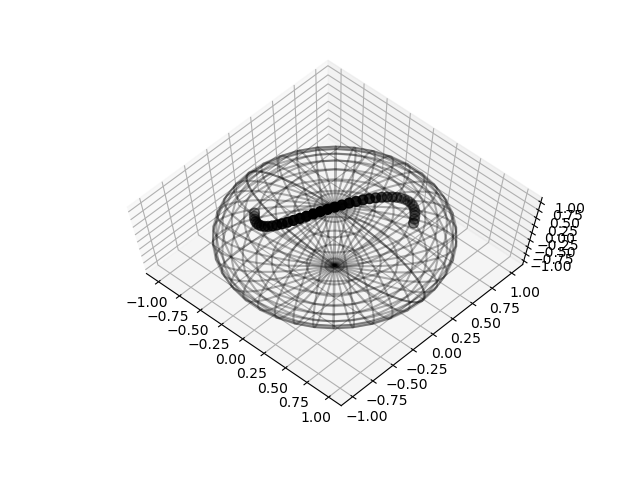
\includegraphics[]{Data_13.png}
        \caption{Toy data 13, $\mathbb{R}^3$}
        \label{fig:toydata}
    \end{center}
\end{figure}

\newpage

For example, this dataset is created by setting the first coordinate of the 
i-th point, $x_{i, 1} = \frac{i-n/2}{n}$, then $x_{i, 2} = sin(4*x_{i, 1})/2$, 
and the third to $x_{i, 3} = \sqrt{1-x_{i, 1}^2 - x_{i, 2}^2}$, 
where n is the number of points we want to generate.\\
Now that we have seen the Toy Data, let us apply the Principal Flow 
algorithm to the data above.

\begin{figure}[h]
    \begin{center}
        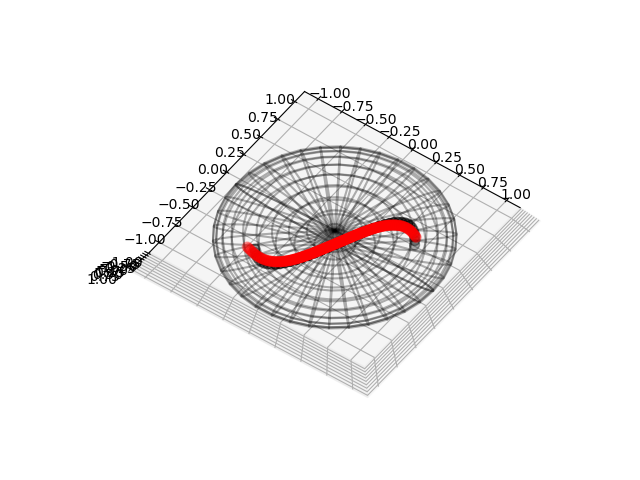
\includegraphics[]{single_flow_13.png}
        \caption{Principal Flow on Toy Data, $\mathbb{R}^3$}
        \label{fig:pflowtoy}
    \end{center}
\end{figure}

This 3D plot shows the original data in black, and the principal flow in 
\textcolor{red}{red}.
With some tuning of h, the size of the neighbourhood, we can see that we have constructed
a principal flow that follows the original data almost
exactly, reconstructing an S with some slight differences at the curves of the s-shape of
the original data.
We have now seen that proof that our principal flow algorithm works:
it is able to accurately reconstruct the toy data, 
the s curve on the sphere.

\subsection{With Noise}

Next, gaussian noise was added to the S-shaped data on the sphere to create a noisy dataset.
Then we fitted a principal flow to this noisy data.
NOte: run noisy flow again! With same seed this time....
\begin{figure}[h]
\centering
\begin{subfigure}{.5\textwidth}
    \centering
    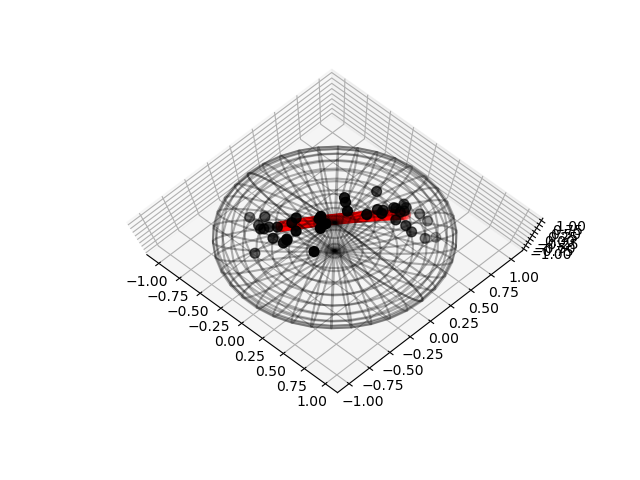
\includegraphics[scale=0.5]{noisy_13.png}
    \caption{Flow on Noisy Data using binary kernel}
    \label{noisybinary}
\end{subfigure}%
\begin{subfigure}{.5\textwidth}
    \centering
    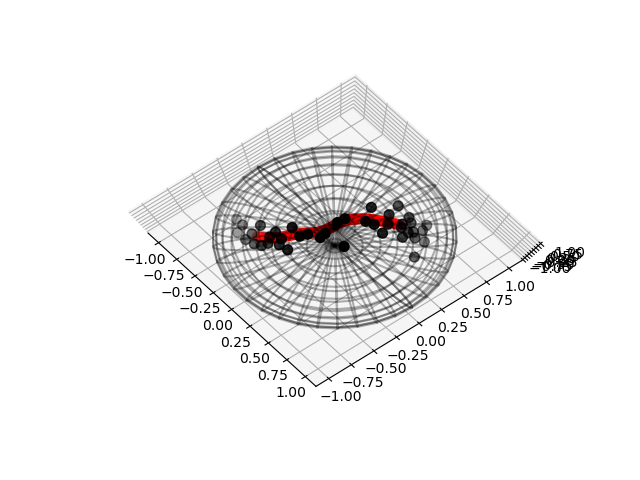
\includegraphics[scale=0.5]{noisy_13_gaussian.png}
    \caption{Flow on Noisy Data using gaussian kernel}
    \label{noisygaussian}
\end{subfigure}
\caption{Illustration of a Tangent Space}
\label{fig:test}
\end{figure}

We can see that the principal flow obtained seems to follow the new pattern 
of variation in the data: from the more dense cloud of points on the left, to the curve of
the points in the center to the other dense cloud of points on the right.
We can see from these examples that even with noise, our algorithm is able to discern 
the pattern of the data.

\subsection{Boundary Flow with Noise}

Next we test out our extension, our algorithm for our principal boundary.
Since we need a "cloud" of data, we apply some gaussian noise on the data from above,
and then run our principal boundary algorithm on it. Let the principal flow
be the curve in red, and the boundaries be in blue and green.

\begin{figure}[h]
    \begin{center}
        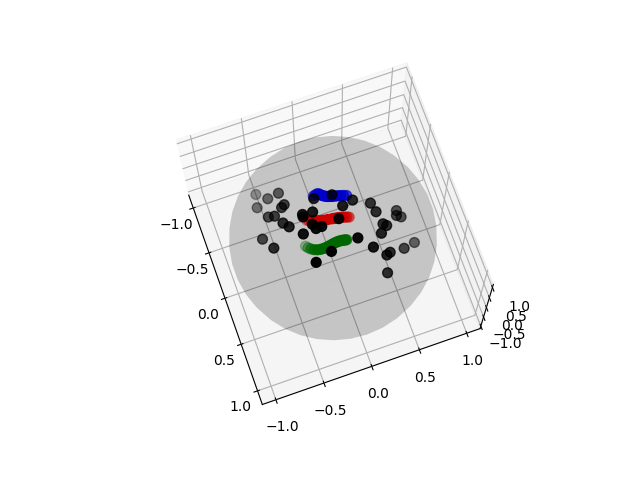
\includegraphics[scale=0.8]{noisy_boundary_flow13.png}
        \caption{Boundary Flow on noisy data}
        \label{fig:boundaryflows}
    \end{center}
\end{figure}

With some tuning, we obtain these 3 curves: we can see that the principal flow
is in the middle of the dataset, while the boundary flows accompany it in parallel
and even form to the shape of the cloud of data, bending outwards
when there is a point beyond it. Through this graph, we can see how the principal
boundary can work and be shaped by the shape of the cloud of data.

\section{Real World Data}

Our results on artificial data are promising, however, it means little
if there are no real-world applications for our greedy principal flow.

\subsection{MNIST}
 
We first test the principal flow algorithm on the MNIST dataset, a rite of passage
for machine learning algorithms. The MNIST dataset is a set of handwritten digits.  

\begin{figure}[h]
    \begin{center}
        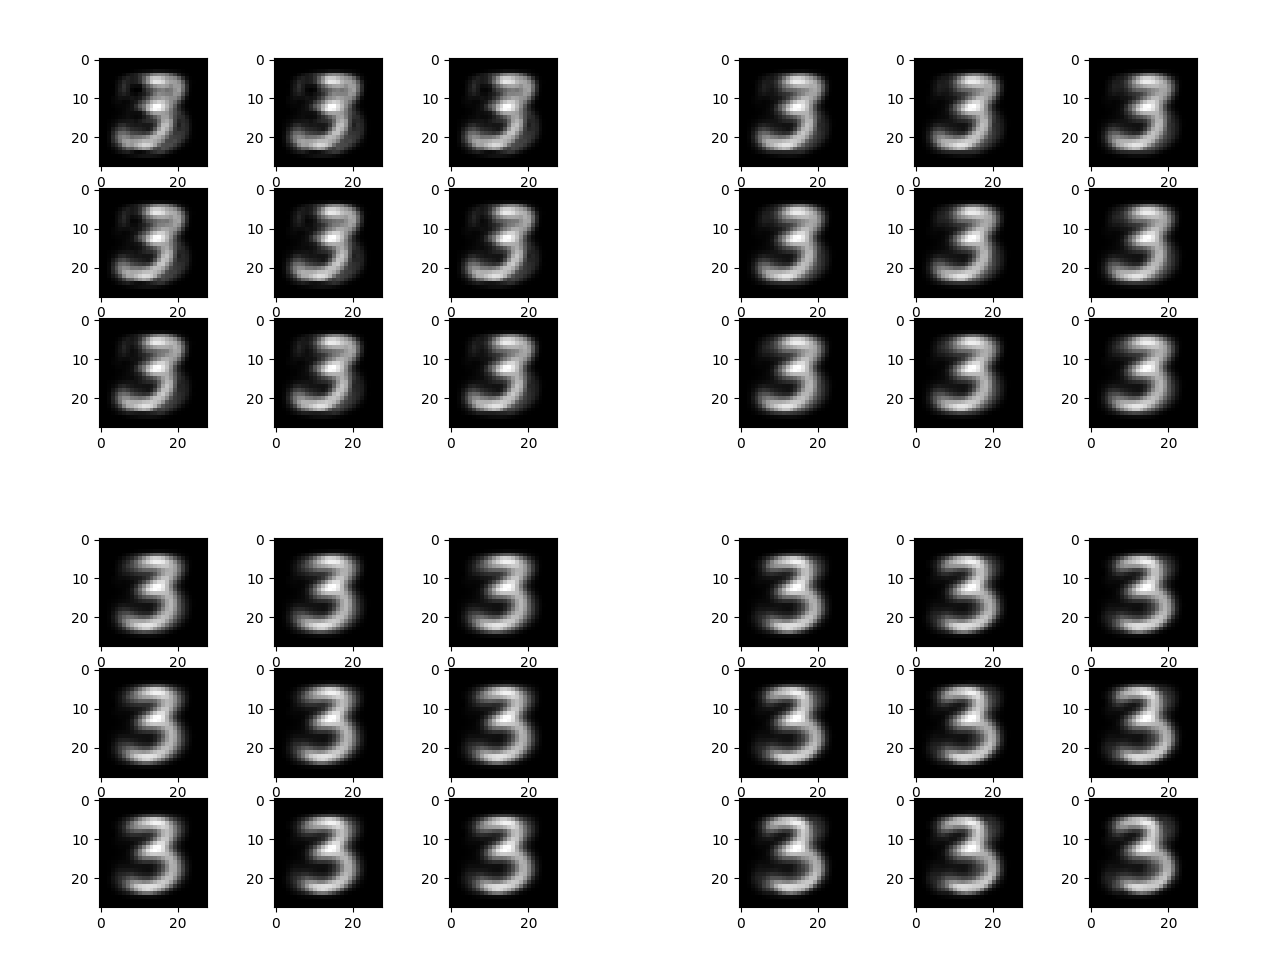
\includegraphics[scale=0.2]{main_mnist.png}
        \caption{MNIST Flows, from left to right.}
        \label{fig:mnistflows}
    \end{center}
\end{figure}

These images, read from left to right, top to bottom, are points from the principal 
flow. Although it does not represent all the variability of the 3s in the dataset, 
we can see that all the images obtained are "nice" representations of 3s, 
in that they cannot be confused with any other digit, and they seem to be relatively
neatly written. Within these "nice" 3s then we observe the source of the variability:
the "slant" of the digit.
We can see that the digits start out leaning right and with a 
which starts out slanting to the right, and slowly rotates
to slant to the left, going through a phase of being perfectly centered. 
This perhaps is an insight into the well-written 3s in the dataset and perhaps 
of neat handwritten digits in general: that they differ mainly in orientation. 
The fact that all the 3s on the principal flow are neat representations of the digit
also suggests that our algorithm has found a path that has some intuitive meaning
we can use to understand our data better, or perhaps that our choice of $\mathcal{M}^d$
was quite appropriate for this dataset.

\subsection{Fashion MNIST}

Next we test our principal flow on objects, and rather on 2 pieces of fashion that
look quite alike: t-shirts and dresses.

\begin{figure}[h]
    \begin{center}
        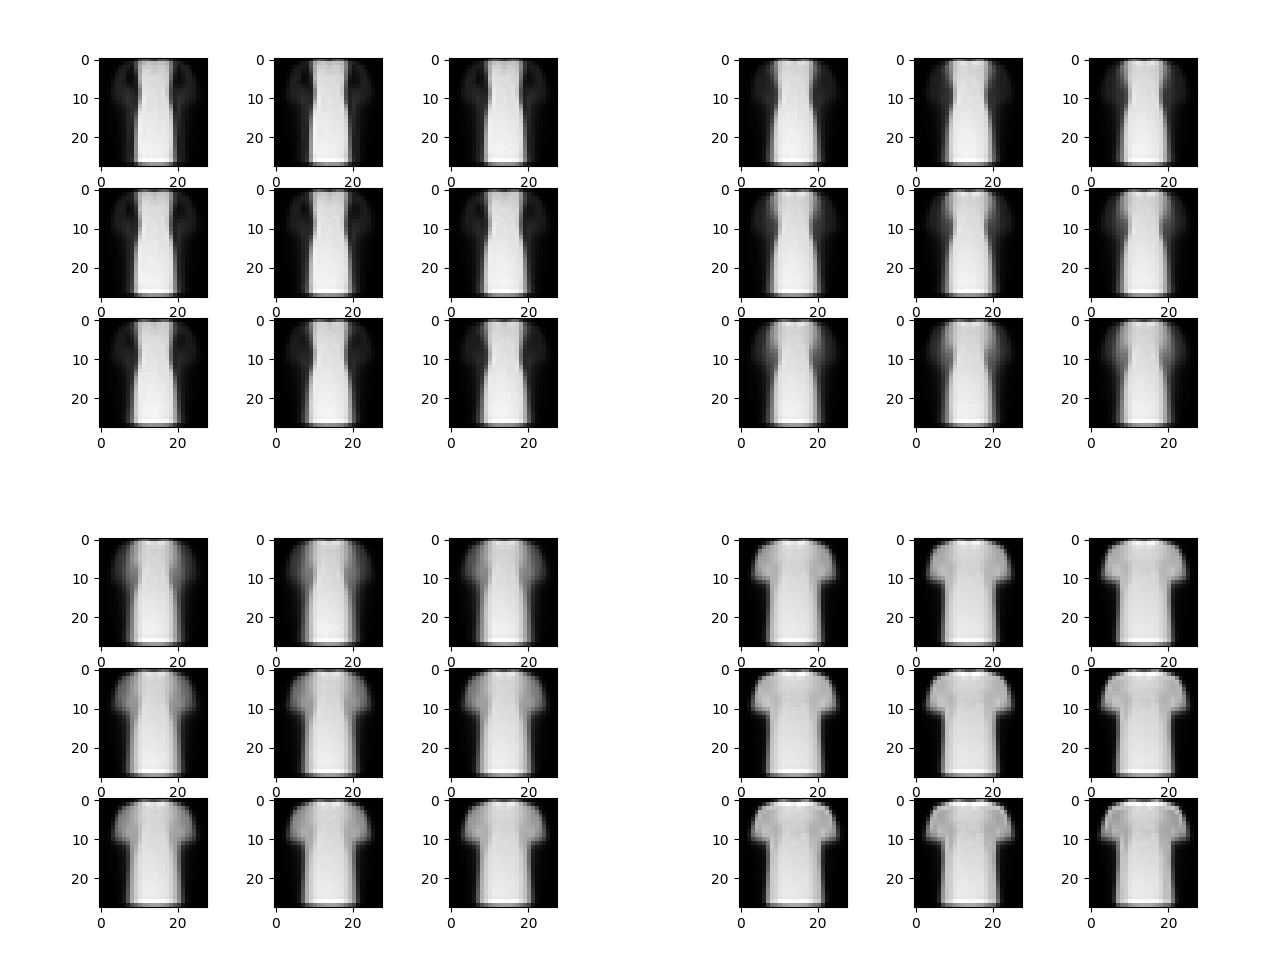
\includegraphics[scale=0.2]{main_fashion.png}
        \caption{Fasion MNIST Flows, from left to right.}
        \label{fig:fashionmnistflows}
    \end{center}
\end{figure}

Here we can watch as dresses morph into t-shirts. More than just an interesting graphic,
it shows that the principal flow is able to capture the variability of the data:
here the data varies very clearly in the outline of the images, and images on the
principal flow reflect this main source of variability.
(do another transition between 2 objects)

\subsection{Olivetti faces}

Next we test our algorithm on a facial dataset. The Olivetti face dataset is old,
and thus images are small, and only in black and white. This however is 
an advantage, as smaller images help the principal flow algorithm run faster,
allowing us to experiment with a variety of parameters.

\begin{figure}[h]
    \begin{center}
        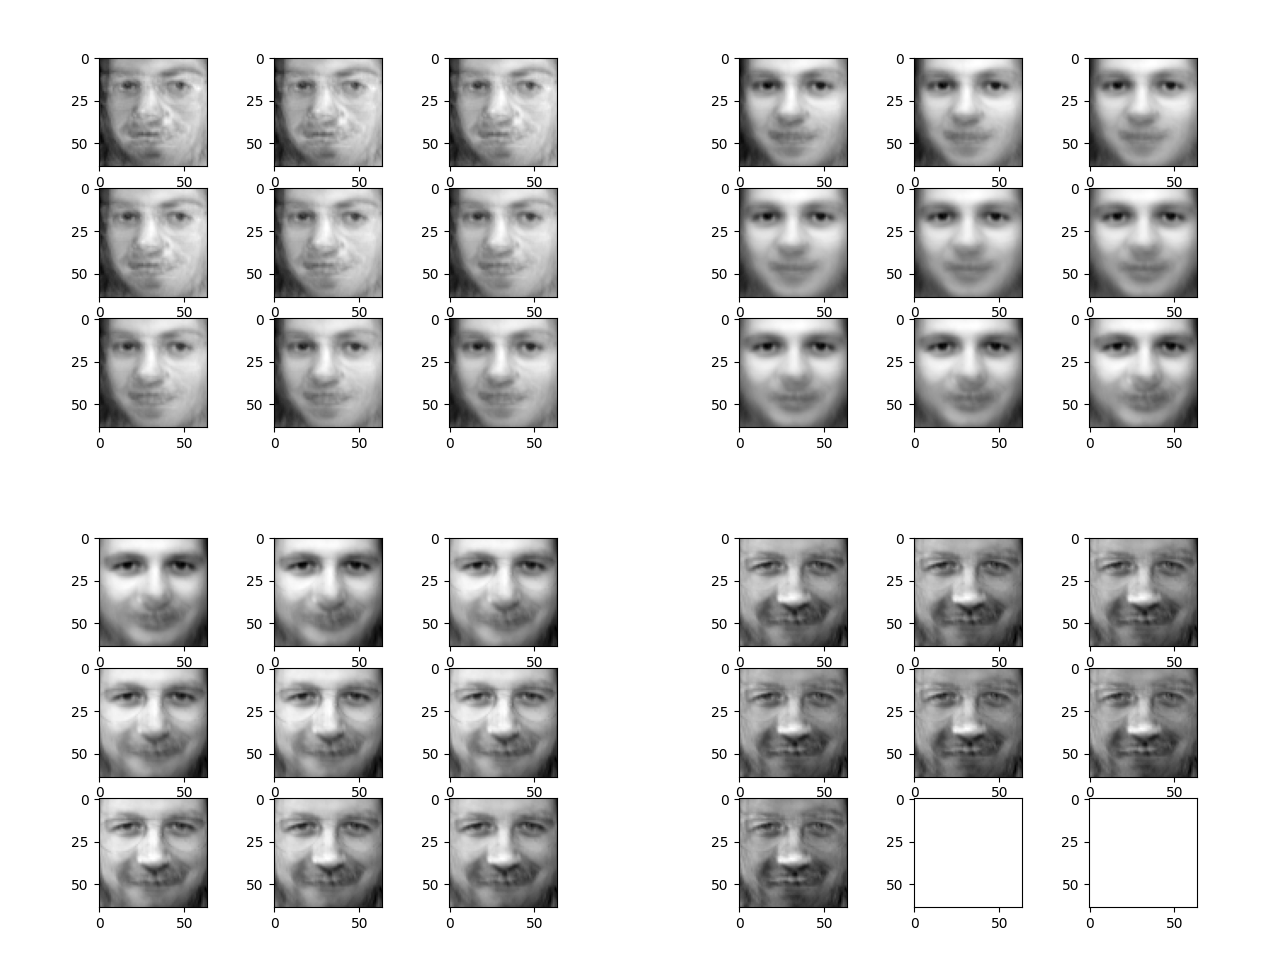
\includegraphics[scale=0.2]{main_olivetti.png}
        \caption{Flow for Olivetti face data, from left to right.}
        \label{fig:olivettiflows}
    \end{center}
\end{figure}

Although disturbing, we can see the results of our algorithm. The pictures we observe 
differ mainly on the angle of their face, and whether they have a beard. Indeed
we observe that the difference between the men and woman in the data are not as stark
as the difference between bearded and non-bearded individuals. 
This again indicates the strength of our algorithm: it is able to suss out the 
main way in which these images vary.
Additionally, we can glean meaning from neighbouring images on the curve:
they are close to each other in a meaningful way. 
We can see the series of faces transition from being slightly tilted away from
the camera to facing the camera directly. The fact that the images on the principal flow
transition smoothly tell us that a face slightly tilted away is near a face directly facing
the camera which makes intuitive, real world sense.
This is an indication that our choice of $\mathcal{M}^d$ does yield fruit and
have some real world meaning, and that our principal flow seems to preserve some
real world interpretation and meaning as it transitions smoothly through the orientation
of faces in the data.

\iffalse
\subsection{Cartoon Faces}

\begin{figure}[h]
    \begin{center}
        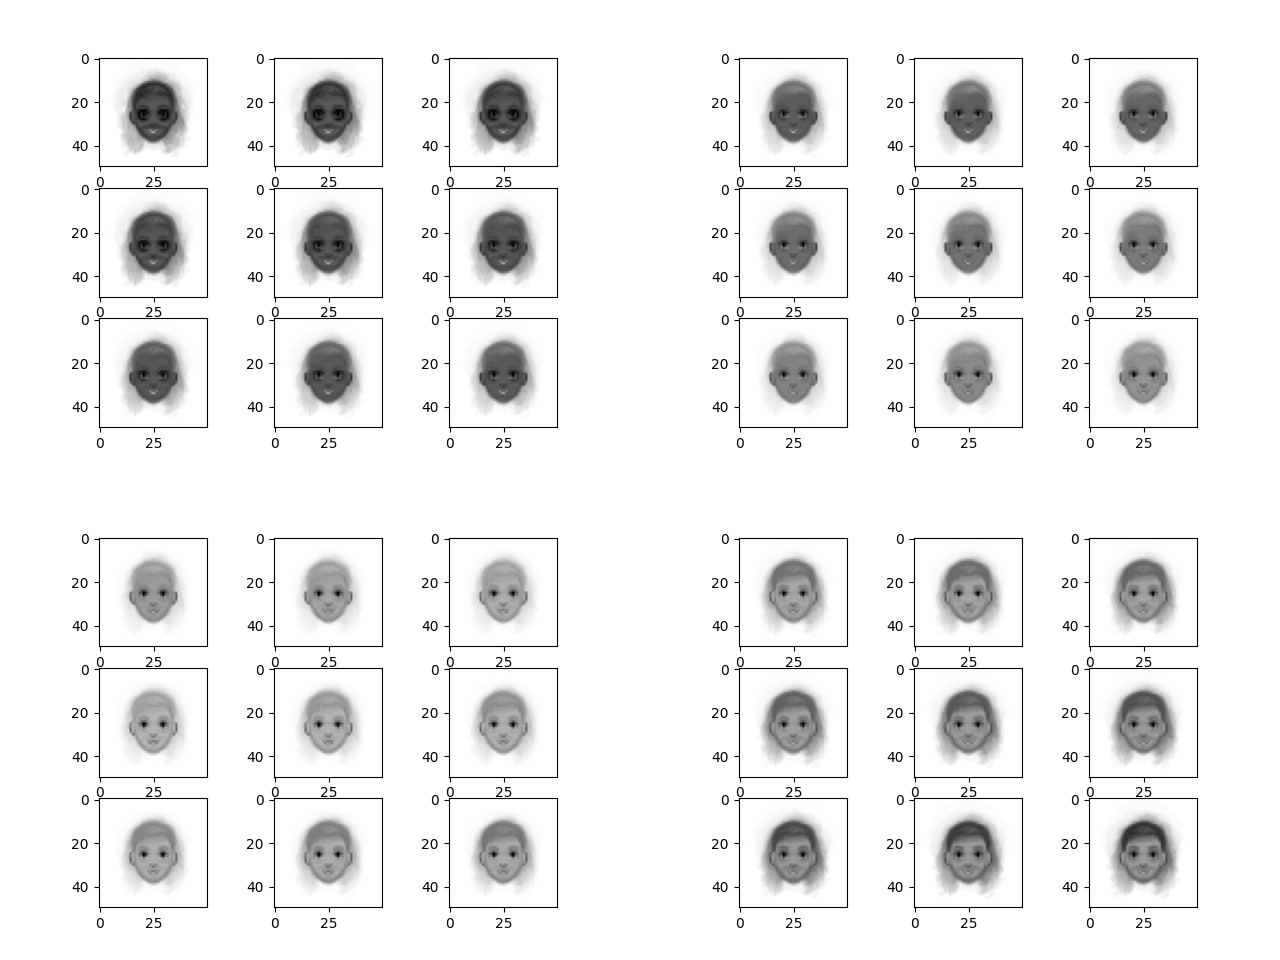
\includegraphics[scale=0.2]{main_cartoon_10_01.png}
        \caption{Cartoon face Flows, from left to right.}
        \label{fig:cartoonfaceflows}
    \end{center}
\end{figure}

When run on a dataset of cartoon faces, the principal flow finds a series of 
faces that differ greatly in skin color and in hair color. Along the flow 
we can see that the faces start with a dark skin color and gradually 
transition to a lighter skin color, then get darker along with their hair color. 
Here we can see that faces vary mainly on skin tone and hair color, which makes intuitive sense, 
since other features like spectacles and a particular hair shape may not feature on many
data points.
\fi
\subsection{Faces in the Wild}
\begin{figure}[h]
    \begin{center}
        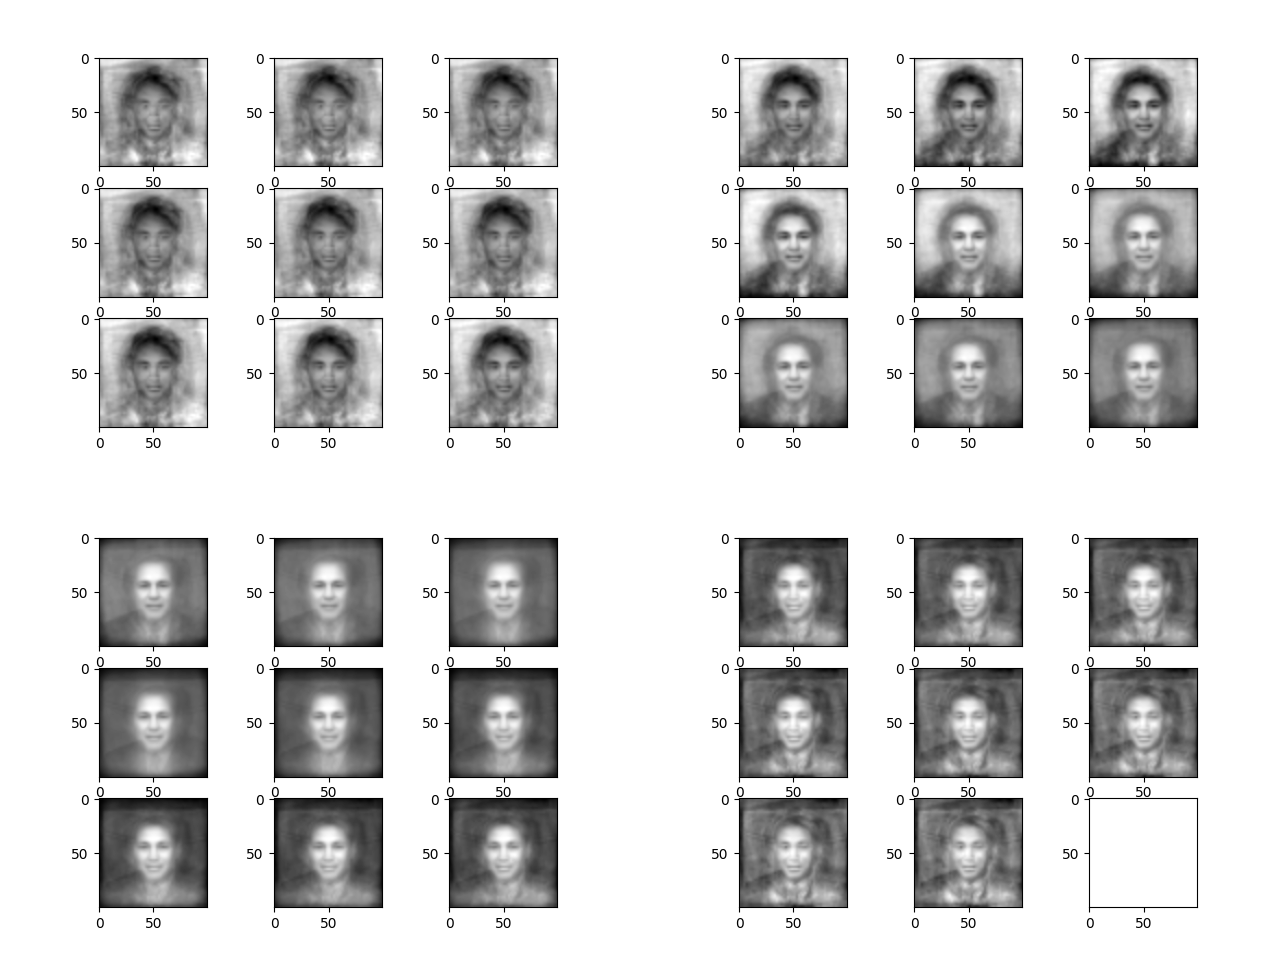
\includegraphics[scale=0.2]{main_lfw_10_05.png}
        \caption{Faces in the wild flow, from left to right.}
        \label{fig:cartoonfaceflows}
    \end{center}
\end{figure}

Here we test our principal flow algorithm on real faces with differing backgrounds, 
since these are photos found online. As with the cartoon faces, we can see that
these faces differ in skin tone but also in eyebrow color, eye shape and background. 
This makes intuitive sense, since skin tone will determine a large portion of the face,
and the background also takes up a large part of the images, and are likely to differ 
quite greatly.


\chapter*{Future Directions}

The topic of principal flows and manifold learning in general is a rich field 
with much potential, and there are many avenues of 
expanding the work done in this report. 
One potential direction is constructing the k-th order principal flows, where $k>1$. 
Another potential avenue of research is using different kinds of $\mathcal{M}^d$. 
In this report, we have restricted ourselves only to the hypersphere. Although this 
might be a "good enough" approximation, if we had intuition about the specific form 
of the manifold on which our multivariate data lies, and we determine that the 
hypersphere is unsuitable, then this current principal flow would not be able to 
accomodate this intuition. With a different manifold, we might be able to obtain 
a different principal flow that might give us more information about the 
variability of the data and describe it more appropriately than using the hypersphere. 
Additionally, we could also extend the greedy principal boundary to be a maximal margin
classifier. Although this has already been done in \cite{principalboundary}, 
it has yet to be done with a greedy approach, and would be the first
greedy maximal margin classifier for multivariate data lying on some 
Riemannian manifold.


\section{Corrections}

\subsection{Abstract}
Abstract too simple: can mention manifold data: higher dimensional mention multivariate
data set: higher dimensional data but can be viewed as lying on a lower dimensional 
manifolds
must explain principal flows in abstract.  
Must talk about hyperspheres more specifically explain why hyperspheres are there
After rotation and centering and translation and normalisation, vectors can be viewed 
as points on the hyperspheres. 

\subsection{Motivation}

seperately talk about programming language stuff in another paragraphed

\subsection{Definitions}

Remove the words denotes. $\mathbb{R}^D$ is the D-dimensional euclidean space. 



\begin{thebibliography}{9}

\bibitem{mds}
Ingwer Borg and Patrick J.F. Groenen (2005) "Modern Multidimensional Scaling"
, \textit{Springer}.

\bibitem{pga}
Fletcher, P. T., Lu, C., Pizer, S. M., and Joshi, S. (2004), "Principal Geodesic Analysis for the
Study of Nonlinear Statistics of Shape," 
\textit{IEEE Transactions on Medical Imaging}, 23, 995-1005.

\bibitem{isomap}
Tenenbaum, J. B., Vin de Silva, and Langford, J. C. (2000). "A Global
Geometric Framework for Nonlinear Dimensionality Reduction." 
\textit{Science}, 290: 2319-2323.

\bibitem{principalboundary}
Yao, Z., and Zhang, Z. (2019) "Principal Boundary on Riemannian Manifolds." 

\bibitem{principalflow}
Panaretos, V. M., Pham, T., and Yao, Z. (2014), 
"Principal Flows," \textit{Journal of the American
Statistical Association}, 109, 424-436.

\bibitem{lle}
Saul, Lawrence K. and Sam T. Roweis (2003). “Think Globally, Fit Locally:
Supervised Learning of Low Dimensional Manifolds.” \textit{Journal of Machine
Learning Research}, 4: 119–155. URL http://jmlr.csail.mit.edu/papers/
v4/saul03a.html.

\bibitem{tanspaceimg}
%https://www.researchgate.net/figure/Tangent-space-of-the-manifold-M-at-point-P-S-i-the-tangent-vector-of-P-i-and_fig1_47408095
%https://www.researchgate.net/figure/Conceptual-illustration-of-the-tangent-space-at-point-P-on-a-Riemannian-manifold-M_fig2_262974373

\end{thebibliography}

\end{document}